\documentclass{beamer}
\usepackage{beamerthemeshadow}
\usepackage{beamercolorthemedolphin}
\usepackage{lastpage}

\usepackage{xcolor}
\usepackage{pgf}

\newcommand{\bi}{\begin{itemize}}
\newcommand{\ei}{\end{itemize}}
\newcommand{\be}{\begin{enumerate}}
\newcommand{\ee}{\end{enumerate}}
\newcommand{\bd}{\begin{description}}
\newcommand{\ed}{\end{description}}
\newcommand{\prbf}[1]{\textbf{#1}}
\newcommand{\prit}[1]{\textit{#1}}
\newcommand{\beq}{\begin{equation}}
\newcommand{\eeq}{\end{equation}}
\newcommand{\bdm}{\begin{displaymath}}
\newcommand{\edm}{\end{displaymath}}

\newcommand{\ft}[1]{
  \frametitle{\begin{tabular}{p{4in}r} #1 & \small{\textcolor{white}{\thepage$~$ / \pageref{LastPage}}}\end{tabular}}
  \setbeamercovered{transparent=18}
}

\newcommand{\stepinv}{\setbeamercovered{invisible}}
\newcommand{\stopinv}{\setbeamercovered{transparent=18}}
\newcommand{\uncoverinv}[1]
{
  \setbeamercovered{invisible}
  \uncover<+->{#1}
  \setbeamercovered{transparent=18}
}
\newcommand{\ans}[1]{\textcolor{blue}{#1}}
\newcommand{\ansinv}[1]
{
  \setbeamercovered{invisible}
  \uncover<+->{\textcolor{blue}{#1}}
  \setbeamercovered{transparent=18}
}
\newcommand{\setinv}{\setbeamercovered{invisible}}
\newcommand{\setvis}{\setbeamercovered{transparent=18}}
\newcommand{\centerpic}[2]
{
  \begin{center}
  \includegraphics[#1]{#2}
  \end{center}
}
\newcommand{\h}[1]{\hat{#1}}
\newcommand{\ds}{\displaystyle}

\definecolor{mycolor}{rgb}{0.125,0.5,0.05}
\usecolortheme[named=mycolor]{structure}

\title[Regime Switching, Learning, and the Great Moderation]{Regime Switching, Learning, and the Great Moderation}
\author[Macro Group Workshop.  Indiana University.  April 2007.]{James Murray}
\date{April 6, 2007}

\begin{document}

\frame{\titlepage}
\setcounter{page}{1}

\frame
{
  \ft{Time Varying Volatility}
    \hspace*{-0.4in}\begin{tabular}{cc}
      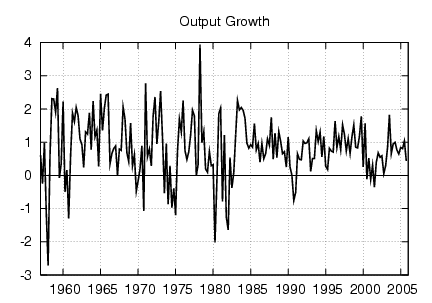
\includegraphics[scale=0.4]{plots/ydata.png} &
      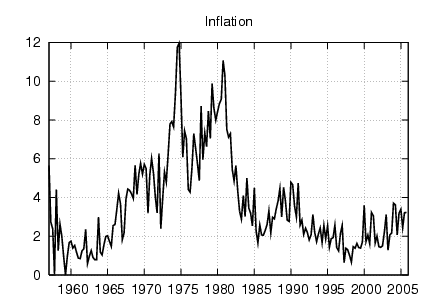
\includegraphics[scale=0.4]{plots/pidata.png} \\
    \end{tabular}
}

\frame
{
  \ft{Competing explanations}
  \bi
  \item Good vs. bad policy.
    \bi
    \item Lubik and Schorfheide (2004): find monetary policy was destabilizing pre-Volker.
    \item Milani (2005): accounting for learning, little evidence of a change in monetary policy 
    \item Primiceri (2005): Monetary authority was optimizing, but mis-informed.
    \ei
  \item Bad luck: bad periods were hit with bad shocks.
    \bi
    \item Sims and Zha (2006): evidence points in favor of bad shocks.
    \item Bullard and Singh (2007): bad luck + Bayesian learning.
    \ei
  \item Learning
    \bi
    \item It is possible for learning \textit{alone} to generate time-varying volatility.
    \item Depends on how you specify learning process.
    \ei
  \ei
}

\frame
{
  \ft{Bad Luck and Learning}
  \bi
  \item Incorporate bad luck and learning into a New Keynesian model.
  \item Estimate how much volatility is explained by these sources.
  \item Marcet and Nicolini (2003) learning.
    \bi
    \item Agents run OLS to form expectations (decreasing learning gain).
    \item If agents suspect structural change, switch to a high learning gain.
    \ei
  \item Bad luck: regime switching in variance of structural shocks.
    \bi
    \item Low volatility regime
    \item High volatility regime
    \ei
  \ei
}

\frame{
  \ft{New Keynesian Model}
  \bi
  \item Continuum of consumer types, each type with a specific labor skill.
  \item Continuum of monopolistically competitive intermediate goods firms.
  \item Calvo (1983) pricing.
  \item No capital.
  \item Taylor rule monetary policy.
  \item Internal habit formation in preferences (mechanical persistence).
  \item Inflation indexation (mechanical persistence).
  \item Serially correlated non-policy shocks: technology and preference.
  \ei
}

\frame
{
  \ft{Consumers}
  \bi
  \item Preferences:
  \beq E_0^* \sum_{t=0}^{\infty} \beta^t \left[ \frac{1}{1-\frac{1}{\sigma}} \xi_t \left(c_t - \eta c_{t-1}\right)^{1-\frac{1}{\sigma}} - \frac{1}{1+\frac{1}{\mu}} n_t(i)^{1+\frac{1}{\mu}} \right] \eeq
  \item Budget constraint:
  \beq c_t + b_t(i) = \frac{1+r_{t-1}}{1+\pi_t} b_{t-1}(i) + \frac{w_t(i)}{p_t} n_t(i) + \Pi_t - \tau_t \eeq
  \item Notation
    \bi
    \item $E_t^*$ denotes a non-rational expectation.
    \item $\xi_t$: preference shock.
    \item $\eta \in (0,1)$: degree of habit formation.
    \item $n_t(i)$ consumer type $i$s choice of labor supply.
    \item $w_t(i)$ nominal wage.
    \item $p_t$, $\pi_t$: price and inflation rate of final good.
    \ei
  \ei
}

\frame
{
  \ft{Intermediate Goods}
  \bi
  \item Intermediate good production: $y_t(i) = z_t n_t(i)$
  \item Calvo (1983) pricing: only a constant fraction, $\omega$ of firms can re-optimize their price each period.
  \item Those who cannot: $p_t(i) = p_{t-1}(i) + \gamma \pi_{t-1}$
  \item Those who can, maximize:
    \beq \label{eq:intprofit}
    E_t^* \sum_{T=0}^{\infty} \left(\omega \beta \right)^{T} \frac{\lambda_{t+T}}{\lambda_t}
    \left\{ \left(\frac{p_{t}(i) \pi_{t+T}^{*}}{p_{t+T}}\right) y_{t+T}(i) - \Psi\left[y_{t+T}(i)\right] \right\}
    \eeq
  \item $\gamma$: degree of inflation indexation.  
  \item Indexation adjustment through period $t+T$:
    \beq \pi_{t+T}^{*} = \prod_{j=1}^{T} (1+\gamma \pi_{t+j-1}) \eeq
  \ei
}

\frame
{
  \ft{Structural shocks}
  \bi
  \item Serially correlated shocks:
  \beq z_t = \rho_z z_{t-1} + \epsilon_{z,t}(s_t) \eeq
  \beq \xi_t = \rho_{\xi} \xi_{t-1} + \epsilon_{\xi,t}(s_t) \eeq
  \item Innovations for a given regime are mean zero and iid.
  \beq \label{eq:vars}
Var\left( \left[ \begin{array}{c} \epsilon_{z,t}(s_t) \\ \epsilon_{\xi,t}(s_t) \end{array} \right] \right) = \left\{
 \begin{array}{c} \left[ \begin{array}{cc} \sigma_{z,1}^2 & 0 \\ 0 & \sigma_{\xi,1}^2 \end{array} \right], \mbox{       if $s_t=1$} \\ 
\left[ \begin{array}{cc} \sigma_{z,2}^2 & 0 \\ 0 & \sigma_{\xi,2}^2 \end{array} \right], \mbox{       if $s_t=2$} \\
\end{array} \right \eeq
  \ei
}

\frame
{
  \ft{Regime Switching}
  \bi
  \item Two state Markov chain
  \item Let $p_i$ denote the probability of staying in regime $i$ from $t-1$ to $t$.
  \item Transition matrix:
    \beq \label{eq:tran} P = \left[ \begin{array}{cc} p_1 & 1-p_1 \\ 1-p_2 & p_2 \end{array} \right]. \eeq
  \ei
}

\frame
{
  \ft{Learning}
  \bi
  \item Log-linearized New Keynesian model has the structural form:
  \beq \label{eq:sform} \Omega_{0} x_t = \Omega_{1} x_{t-1} + \Omega_{2} E_t^* x_{t+1} + \Psi \epsilon_t(s_t) \eeq
  \item All observable by the agents: $x_t = [\h{y}_t~ \pi_t~ \h{r}_t~ \h{z}_t~ \h{\xi}_t]'$
  \item Shocks not observable: $\epsilon_t(s_t) = [\epsilon_{z,t}(s_t)~ \epsilon_{\xi,t}(s_t)~ \epsilon_{r,t}]'$
  \item Rational expectations solution:
  \beq \label{eq:msvsol} E_t x_{t+1} = G x_{t}, \eeq
  \item Agents estimate $G$ by least squares.
    \bi
    \item Use as regressors a constant, and all past observations of $x_t$.
    \ei
  \ei
}

\frame
{
  \ft{Recursive algorithm}
  \bi
  \item It can be shown that least squares implies recursion:
  \beq \label{eq:lnG} \hat{G}_t^* = \hat{G}_{t-1}^* + g_t (x_{t-1} - \hat{G}_{t-1}^* x_{t-2}^*) {x_{t-2}^*}' R_t^{-1} \eeq
  \beq \label{eq:lnR} R_t = R_{t-1} + g_t (x_{t-2}^* {x_{t-2}^*}' - R_{t-1}) \eeq
  \item OLS: $g_t = 1 / (t-1)$
    \bi
    \item Learning dynamics disappear over time.
    \item No suspicion of structural change.
    \item Extremely slow to adjust to structural changes.
    \ei
  \item Constant gain learning: $g_t = g$ for all $t$.
    \bi
    \item Bullard and Duffy (2005)
    \item Time varying volatility is likely small.
    \ei
  \ei
}

\frame
{
  \ft{Endogenous learning gain}
  \bi
  \item Marcet and Nicolini (2003): learning is endogenous.
  \item Let $\alpha_t \equiv 1/g_t$.  In OLS case $\alpha_t$ is sample size.
  \ei
  \beq \label{eq:mngain} \alpha_t = \left\{ \begin{array}{cl} \ds \alpha_{t-1} + 1 & \ds \mbox{     if  } \frac{1}{J} \sum_{j=1}^{J} \frac{1}{n} \sum_{v=1}^{n} \left| \frac{x_{t-j}(v) - \hat{G}_{t-j}^*(v) x_{t-j-1}^*}{\hat{G}_{t-j}^*(v) x_{t-j-1}^*} \right| < \nu \\
  \ds \alpha & \ds \mbox{     otherwise} \end{array} \right \eeq
    
  \bi
  \item Notation:
    \bi
    \item $n$ is the number of variables in $x_t$.
    \item $x_{t-j}(v)$: $v$th element of $x_{t-j}$
    \item $\hat{G}_{t-j}^*(v)$: $v$th row of $\hat{G}_{t-j}^*(v)$
    \item $\alpha \equiv 1/g$ is the constant gain.
    \item $\nu \in (0,\infty)$ is a threshold level.
    \ei
  \ei
}

\frame
{
  \ft{State-space form}
  \bi
  \item State equation:
  \ei
  \beq \label{eq:state} \begin{array}{c}
\ds x_t = b_t + F_t x_{t-1} + v_{t}(s_t) \\ \\
\ds b_t = \Omega_0^{-1}\Omega_{2}\left(I+\h{G}_t\right)\h{g}_{0,t} \\ \\
\ds F_t = \Omega_0^{-1} \left(\Omega_{1} + \Omega_{2} \h{G}_t^2 \right) \\ \\
\ds v_t(s_t) = \Omega_0^{-1} \Psi \epsilon_t(s_t) \\ \\
\ds Var\left[v_{t}(s_t)\right] = \left( \Omega_0^{-1} \Psi \right) Var\left[\epsilon_t(s_t)\right] \left(\Omega_0^{-1} \Psi\right)' 
  \end{array} \eeq
  \bi
  \item Observation equations:
  \beq \begin{array}{c} \label{eq:obs}  
  \ds GDP_t = 100 \h{y}_t, \\
  \ds INF_t = \pi^{*} + 400\pi_t, \\
  \ds FF_t = r^{*} + 400\h{r}_t,
  \end{array}
  \eeq
  \ei
}

\frame
{
  \ft{Parameters to Estimate}
  \bi
  \item New Keynesian model parameters.
  \item Variance of the shocks in each state: $\sigma_{z,1}^2, \sigma_{\xi,1}^2$, and $\sigma_{z,1}^2, \sigma_{\xi,1}^2$.
  \item Probabilities of switching between states: $p_1$, $p_2$.
  \item Learning parameters: $g$ and $\nu$.
  \ei
}


\frame
{
  \ft{Estimation}
  \bi
  \item Kim (1994), Kim and Nelson (1999): form the likelihood.
    \bi
    \item Kalman filter for state-space models.
    \item Hamilton (1989) filter for regime switching.
    \ei
  \item Plan to estimate:
    \bi
    \item Smoothed estimates of the regime probabilities for each period.
    \item Learning gain for each period.
    \item Smoothed estimates of the shocks.
    \item Out-of-sample forecasts of the model.
    \ei
  \ei
}

\frame
{
  \ft{Interesting questions}
  \bi
  \item With endogenous gain learning, how sizable of an increase in shock volatility is necessary to explain volatile periods such as the 1970s.
  \item When did regime changes occur? 
  \item When did learning gain changes occur?
  \item How do these answers compare to constant gain learning, decreasing gain learning, and rational expectations.
  \item How well does do competing specifications fit the data.
    \bi
    \item Different assumptions on learning gain.
    \item Fixed state regime.
    \ei
  \ei
}

\end{document}

